%!TEX root = ../synopsis.tex

\section*{ОСНОВНОЕ СОДЕРЖАНИЕ РАБОТЫ}
Во {\bf введении}
обосновывается актуальность диссертационной работы,
определены цель и задачи исследования,
представлена научная новизна, теоретическая и практическая значимость работы.
Приведены основания для выполнения работы, ее апробация и структура.


%!TEX root = ../synopsis.tex

В {\bf первой главе}
проводится анализ проблемы автоматизированного проектирования УП
в раскройно-заготовительном производстве для оборудования термической фигурной резки с ЧПУ.
Описаны основные технологические особенности и ограничения термической резки,
которые необходимо соблюдать при проектировании УП.

\begin{figure}[h]
  \centering
  \includegraphics[width=0.8\textwidth]{toolpath.pdf}
  \caption{Элементы маршрута резки}
  \label{fig:toolpath}
\end{figure}

В общем случае маршрут инструмента содержит несколько компонент:
начальную $M_0$
и возможно отличную от неё конечную точку маршрута $M_{N+1}$,
$N$~точек врезки $M_i$, $i \in \overline{1, N}$
и соответствующих им точек выключения инструмента
$M_i^*$,
рабочий ход инструмента от точки врезки $M_i$
до точки выключения $M_i^*$
(в дальнейшем будем называть его траекторию
{\it сегментом резки}
$S_i=M_i M_i^*$)
а также холостой ход от $M_i^*$
до следующей точки врезки $M_{i+1}$,
см. рис.~\ref{fig:toolpath}.
В определение маршрута также входит
порядок резки,
то есть последовательность посещения точек врезки,
представляющая собой перестановку
$I = (i_1, i_2, ... i_N)$.
Таким образом,
маршрут резки можно определить
в терминах сегментов резки как кортеж
\begin{equation}
  \mathfrak{R} = \left<
    M_0, M_1, S_1, M_1^*, M_2, S_2, M_2^*, \,\dots, M_N, S_N, M_N^*,
    i_1, i_2, \,\dots, i_N
  \right>
  \label{eq:route:tuple}
\end{equation}

В качестве целевой функции при оптимизации часто используется время резки
\begin{equation}
  T_{cut} = \frac{L_{on}}{V_{on}} + \frac{L_{off}}{V_{off}} +N_{pt} \cdot t_{pt}
  ,
  \label{eq:cutting-time}
\end{equation}
где
$L_{on}$ -- длина реза с включенным режущим инструментом;
$V_{on}$ -- скорость рабочего хода режущего инструмента;
$L_{off}$ -- длина переходов с выключенным режущим инструментом (холостой ход);
$V_{off}$ -- скорость холостого хода;
$N_{pt}$ -- количество точек врезки;
$t_{pt}$ -- время, затрачиваемое на одну врезку.
В подавляющем большинстве исследований,
включая данную диссертационную работу,
$V_{on}$ считается константой
(в рамках конкретной УП),
однако вообще говоря это не так,
см.~\cite{Obuhovo}.

Важнейшей экономической характеристикой качества
разработанной управляющей программы является стоимость
(себестоимость) резки деталей на машине с ЧПУ.
По аналогии с \eqref{eq:cutting-time}
его можно определить по формуле:
\begin{equation}
  F_{cost}=
  L_{on} \cdot C_{on} +
  L_{off} \cdot C_{off} +
  N_{pt} \cdot C_{pt}
  ,
  \label{eq:cutting-cost}
\end{equation}
где
$C_{on}$ -- стоимость единицы пути с включенным режущим инструментом;
$C_{off}$ -- стоимость единицы пути с выключенным режущим инструментом;
$C_{pt}$ -- стоимость одной врезки.

Задача оптимизации маршрута инструмента для машин фигурной листовой резки с~ЧПУ
может быть представлена в общем виде
как задача минимизации некоторой числовой функции
$\mathfrak F$
(например, \eqref{eq:cutting-time} или \eqref{eq:cutting-cost})
на множестве
$\mathfrak G$ допустимых кортежей
\eqref{eq:route:tuple}:
\begin{equation}
  \mathfrak F(\mathfrak R) \to \min_{\mathfrak R \in \mathfrak G}
  \label{eq:cut:problem}
\end{equation}

В маршрут \eqref{eq:route:tuple} помимо перестановки
$I = (i_1, i_2, ... i_N)$.
входят также точки $M_i$ и $M_i^*$,
которые в общем случае должны ещё быть выбраны
из некоторого непрерывного множества,
что делает простую формулировку задачи \eqref{eq:cut:problem}
чрезвычайно сложной в решении.
Более того,
набор сегментов резки $S_i$
в общем случае не совпадает
(даже в количестве)
с набором контуров деталей,
подлежащих резке,
так как на практике используются различные техники резки:
\begin{enumerate}
  \item
  {\it Резка по замкнутому контуру (стандартная техника)}:
  в этом случае сегмент резки содержит
  ровно один замкнутый контур заготовки,
  который вырезается целиком.
  \item
  {\it Мультисегментная резка контура}:
  в этом случае для вырезки одного контура
  используются не менее двух сегментов резки.
  \item
  {\it Мультиконтурная резка}:
  резка предполагает вырезку нескольких
  контуров в одном сегменте.
\end{enumerate}

На рис.~\ref{fig:cut-classes}
представлена классификация задач резки\dots


\begin{figure}
  \centering
  \includegraphics[width=0.95\textwidth]{classes.pdf}
  \caption{Классификация задач резки}
  \label{fig:cut-classes}
\end{figure}

%!TEX root = ../synopsis.tex

В {\bf третьей главе} 
рассматривается обобщённая задача коммивояжера с
ограничениями предшествования ({\it PCGTSP}) --
это хорошо известная задача комбинаторной оптимизации,
имеющая множество приложений помимо
оптимизации траектории режущего инструмента 
и привлекшая внимание многих исследователей.
К сожалению,
в отличие от задачи GTSP,
алгоритмические подходы к решению 
именно PCGTSP всё ещё малочисленны.
Алгоритм, предложенный в данной диссертационной работе,
на основе синтеза нескольких идей других исследователей,
представляет собой попытку
создать первый точный алгоритм 
ветвей и границ для
решения задачи PCGTSP в общем виде.

Задача определяется тройкой
$(G,\mathcal C,\Pi)$, 
где
$G=(V,E,c)$ -- взвешенный ориентированный граф на $n$
вершинах,
задающий веса $c(u,v)$ для всех своих ребер
$(u,v)\in E, u, v \in V$;
$\mathcal C=\{V_1,\ldots,V_m\}$ -- разбиение вершин
графа $G$ на $m$ кластеров;
$ \Pi = (\mathcal C, A) $ -- частичный порядок,
заданный на множестве кластеров.
Для каждой вершины 
$v\in V$, за $V(v)$ 
обозначим (единственный) кластер 
$V_p\in\mathcal C$, 
такой что
$v\in V_p$. 

Допустимым решением задачи
$(G,\mathcal C,\Pi)$
называется тур (замкнутый путь) $T$,
удовлетворяющий условиям:
\begin{itemize}
    \item 
    имеет длину $|T|=m$
    \item
    начинается и заканчивается в некоторой вершине $v_1\in V_1$
    \item 
    посещает каждый кластер $V_p\in\mathcal C$
    \item
	каждое ребро
	$(v_i, v_j)$ в $T$ 
	(кроме ребра $(v_m,v_1)$) 
	удовлетворяет ограничению предшествования,
	то есть
	 $(V(v_i),V(v_j))\in A$.
\end{itemize}

Каждому решению
$T=v_1, v_2, \ldots, v_m$
мы назначаем стоимость
\begin{equation}
    \label{eq:pctgsp-cost}
	cost(T) = c(v_m,v_1) + \sum_{i=1}^{m-1} c(v_i,v_{i+1})
\end{equation}

Требуется найти допустимый тур 
$ T $ 
с минимальной стоимостью
$$ 
cost (T) \to \min_T 
$$

Ключевой идеей алгоритма является построение нижней оценки стоимости решения.
Для этого в каждой вершине дерева поиска исходная задача разделяется на две:
\begin{enumerate}
    \item 
    Фиксируется {\it префикс}
    маршрута $\sigma=\{V_1, \dots, V_r\}$.
    Обозначим $c_{min}$ нижнюю границу длины
    всех путей, проходящих из вершин кластера $V_1$
    в вершины кластера $V_r$ строго в порядке $\sigma$.
    \item 
    Построим вспомогательную задачу $\mathcal P$,
    удалив из исходной задачи все кластеры,
    являющиеся внутренними в $\sigma$ и 
    соединив все вершины из $V_1$ с вершинами $V_r$
    ребрами нулевого веса.
    Полученная таким образом задача всё ещё сложна,
    однако она может быть несколькими способами
    упрощена (релаксирована) $\mathcal P \to \mathcal P_{rel}$
    и для неё найдено оптимальное решение $\mathrm{OPT}(\mathcal P_{rel})$
\end{enumerate}
Нижняя оценка $LB$
находится как
\begin{equation}
    \label{eq:pcgtsp-lb}
    LB = c_{\min} + \mathrm{OPT}(\mathcal P_{rel})
\end{equation}

В качестве релаксации $\mathcal P_{rel}$ задачи $\mathcal P$
могут применяться:
\begin{itemize}
    \item 
    хорошо известная трансформация Noon-Bean,
    преобразующая задачу GTSP в обычную задачу
    коммивояжера TSP
    \item
    построение вспомогательного {\it графа кластеров} $H_1$
    с весами, индуцированными весами исходного графа $G$:
    $$
    c(V_i, V_j) = \min_{v_i \in V_i, v_j \in V_j} c(v_i, v_j)
    $$
    \item
    построение графа кластеров $H_2$, 
    веса в котором также индуцированы весами путей длины 2 в исходном графе $G$:
    $$
    c(V_i, V_j) = 
        \min_{\substack{v_i \in V_i, v_j \in V_j\\v_k \notin V_i \cup V_j}  } 
        \frac{c(v_i, v_k) + c(v_k, v_j)}{2}
    $$
    при этом маршрут $v_i, v_k, v_j$ должен удовлетворять ограничению предшествования $\Pi$.
    Этот способ позволяет точнее учитывать взаимное расположение контуров на плоскости
    в случае Евклидовой задачи PCGTSP
    \item 
    по аналогии с $H_2$ могут строиться кластерные графы с весами на основе
    путей большей ($\geqslant 3$) длины,
    однако алгоритм их расчёта существенно сложнее и
    не входит в рамки данной диссертационной работы
\end{itemize}

Наконец, для (быстрого) поиска
нижней оценки на решение задачи $TSP(\mathcal P_{rel})$
можно использовать:
\begin{itemize}
    \item 
    Решение задачи о минимальном остовном дереве
    (Minimal Spanning Arborescence, MSAP),
    так как $MSAP(\mathcal P) \leqslant TSP(\mathcal P)$
    \item
    Решение задачи о цикловом покрытии (Cycle cover);
    оно находится как решение задачи о назначениях
    (Assignment Problem, AP) 
    для двудольного графа,
    обе доли которого представляют $\mathcal P_{rel}$;
    опять $AP(\mathcal P) \leqslant TSP(\mathcal P)$
    \item
    в некоторых случаях можно прямо решить задачу 
    коммивояжера $TSP(\mathcal P)$.
    В данной работе для этого использовался решатель Gurobi
    и MIP-модель ATSPxy.
\end{itemize}

Все возможные методы оценки нижней границы показаны в табл.~\ref{t:LBs},
используемые в описываемой реализации обозначены
$L_1$--$L_3$,
не используемые -- 
$E_1$--$E_6$.
Проведённые численные эксперименты показывают,
что часть методов
($E_1$--$E_4$)
систематически дают более слабые оценки,
а часть
($E_1$--$E_2$, $E_5$--$E_6$)
требуют значительных временных затрат по сравнению с выбранными.
Оценка $L_3$ 
в этом смысле является компромиссом,
причём она вычисляется только для малой доли
префиксов
($\approx 1\%$)
с наименьшей оценкой, полученной методами
$L_1$--$L_2$.


\begin{table}
    \centering
    \caption{Методы оценки нижней границы}\label{t:LBs}
    \begin{tabular}[t]{*{5}{|c}|}
        \hline
        & \textbf{Noon-Bean} & $\mathbf{H_1}$ & $\mathbf{H_2}$ & $\mathbf{H_{3+}}$\\
        \hline \hline
      \textbf{AP} & $E_1$ & $\mathbf{L_1}$ & $\mathbf{L_2}$ & - \\
      \textbf{MSAP} & $E_2$ & $E_3$ & $E_4$ & - \\
      \textbf{Gurobi} & $E_5$ & $\mathbf{L_3}$ & $E_6$ & -\\ 
      \hline 
    \end{tabular}    
\end{table}
%!TEX root = ../synopsis.tex

Во {\bf второй главе} 

%!TEX root = ../synopsis.tex

В {\bf четвёртой главе}
рассматривается методология
использования алгоритмов решения
разных классов задачи резки в существующих
CAD/CAM-системах на примере
САПР~<<Сириус>>.
Поскольку требуется обеспечить
совместную работу программного обеспечения,
разработанного в разное время разными командами разработчиков,
чрезвычайно важными становятся вопросы
организации эффективных программных интерфейсов.

Например, для хранения и обмена геометрической информацией
в САПР~<<Сириус>>
используется унаследованный двоичный формат DBS
\autocite{bi:DBS},
который обладает важными достоинствами:
\begin{itemize}
  \item
  эффективное хранение больших данных за счёт эффективного хранения массивов вещественных
  \item
  возможность добавления новых типов записей для хранения ранее не предусмотренной информации;
  расширяемость формата
  \item
  механизм создания копий деталей и геометрических преобразований над ними.
\end{itemize}

В то же время,
работа с ним сопряжена с рядом сложностей,
прежде всего:
\begin{itemize}
  \item
  Сложность чтения двоичного формата,
  особенно в некоторых языках программирования
  \item
  Структура DBS-файла,
  предназначенная для эффективного хранения,
  сильно отличается от удобного внутреннего представления
  геометрии;
  требуется нетривиальное преобразование при чтении файла
  \item
  Формат DBS создавался в том числе для экономии памяти,
  как дисковой, так и оперативной,
  что более неактуально;
  отказ от этого позволяет резко упростить процедуры экспорта--импорта.
\end{itemize}

В рамках данной диссертационной работы
в целях упрощения взаимодействия различных подсистем
было принято решение использовать по возможности
открытые текстовые форматы для хранения и передачи данных.
В качестве основного формата был выбран формат
JavaScript Object Notation
\autocite{bi:JSON}
(JSON),
ввиду того, что
он с одной стороны имеет готовые библиотеки для чтения и записи
для практически всех современных языков
программирования,
является стандартом де-факто во многих
современных приложениях для обмена данными,
довольно прост,
настолько, что может например,
формироваться даже без использования специализированных библиотек,
но при этом достаточно выразителен.


% \lstinputlisting[
%     language=Java,
%     basicstyle=\footnotesize,
%     showstringspaces=false,
%     numbers=left,
%     captionpos=b,
%     caption=JSON-Схема для DBS-файлов
%     ]
%     {media/dbs.json}


В {\bf заключении}
сформулированы основные научные и практические результаты
диссертационной работы.

В {\bf приложении}
приведены
JSON-схемы разработанных
в ходе работы форматов файлов.

